\documentclass{beamer}

\usepackage[T1]{fontenc}
\usepackage[utf8]{inputenc}
\usepackage{color}
\usepackage{ifxetex}
\usepackage{fancyvrb}
\usepackage{lmodern}
\usepackage{minted}
\usepackage{graphicx}
\usepackage{tikz}
\usepackage{verbatim}
\usetheme{metropolis}
\graphicspath{ {./image/} }

\ifxetex
\usepackage[slantfont,boldfont]{xeCJK}
\setCJKmainfont{"SimHei"}
\setCJKmonofont{"SimHei"}
\XeTeXlinebreaklocale "Hz"
\XeTeXlinebreakskip = 0pt plus 1pt
\fi

\title{r2cLEMENCy}
\subtitle{Build plugins to support the cLEMENCy architecture}
\date{\today}

\author[maskray]{MaskRay}
\institute{r2con 2017}

\begin{document}

\maketitle

\begin{frame}{whoami}
  \begin{itemize}
  \item MaskRay (\ifxetex 宋方睿\fi Sòng Fāng-ruì)
  \item \url{https://maskray.me} Twitter @HaskRay
  \item Software Engineer, San Francisco Bay Area, California, US
  \item Member of \alert{Tea Deliverers} (CTF team)
  \item DEF CON 21$\sim$25 CTF Finals (21$\sim$23 blue-lotus, 24 b1o0p, 25 Tea-Deliverers)
  \item Sadly my RE skill has not improved much over the years\ldots
  \end{itemize}
\end{frame}

\begin{frame}{Tea Deliverers}
  \begin{itemize}
  \item Tea Deliverers = blue-lotus + Nu1L + 110066 + Chaitin Tech
  \item Chinese \url{https://maskray.me/blog/2017-08-01-defcon-25-ctf}
  \end{itemize}
\end{frame}

\begin{frame}{DEF CON 25 CTF Finals}
  \begin{center}
    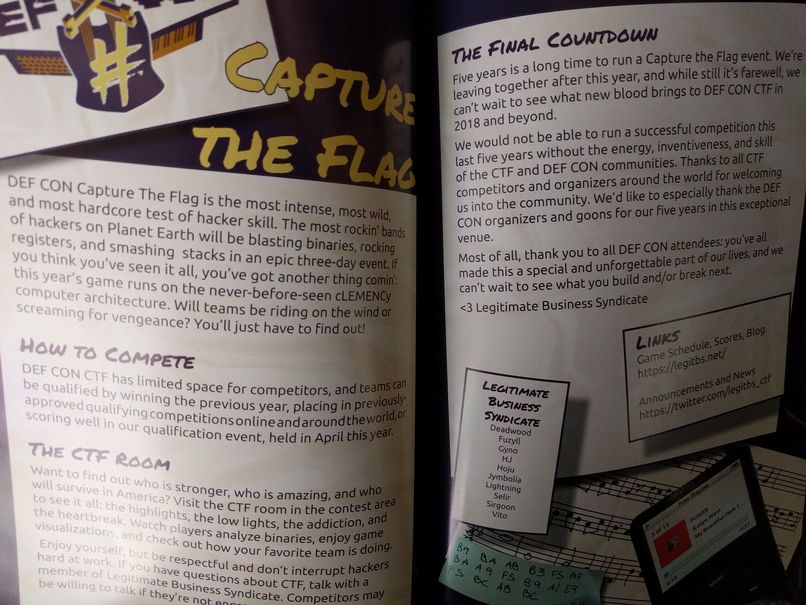
\includegraphics[height=5cm]{defcon-ctf.jpg}
  \end{center}
  \begin{center}
    Curtain call of 5-year organizer Legitimate Business Syndicate
  \end{center}
\end{frame}

\begin{frame}{cLEMENCy}
  \begin{itemize}
  \item Architecture developed by Lightning
  \item 1 `byte' ({\color{blue}nyte}) = \alert{9 bits}
  \item 32 \alert{27-bit} registers + 1 flags register (Zero,Carry,Overflow,Sign+others)
  \item ST=r29 (stack register), RA=r30 (link register), PC=r31, r28 (frame register)
  \item \alert{middle-endian}
  \item \url{https://github.com/legitbs/cLEMENCy}
  \item \url{https://blog.legitbs.net/2017/07/def-con-ctf-2017-final-scores-and-data.html}
  \end{itemize}
\end{frame}

\begin{frame}{cLEMENCy manual}
  \begin{center}
    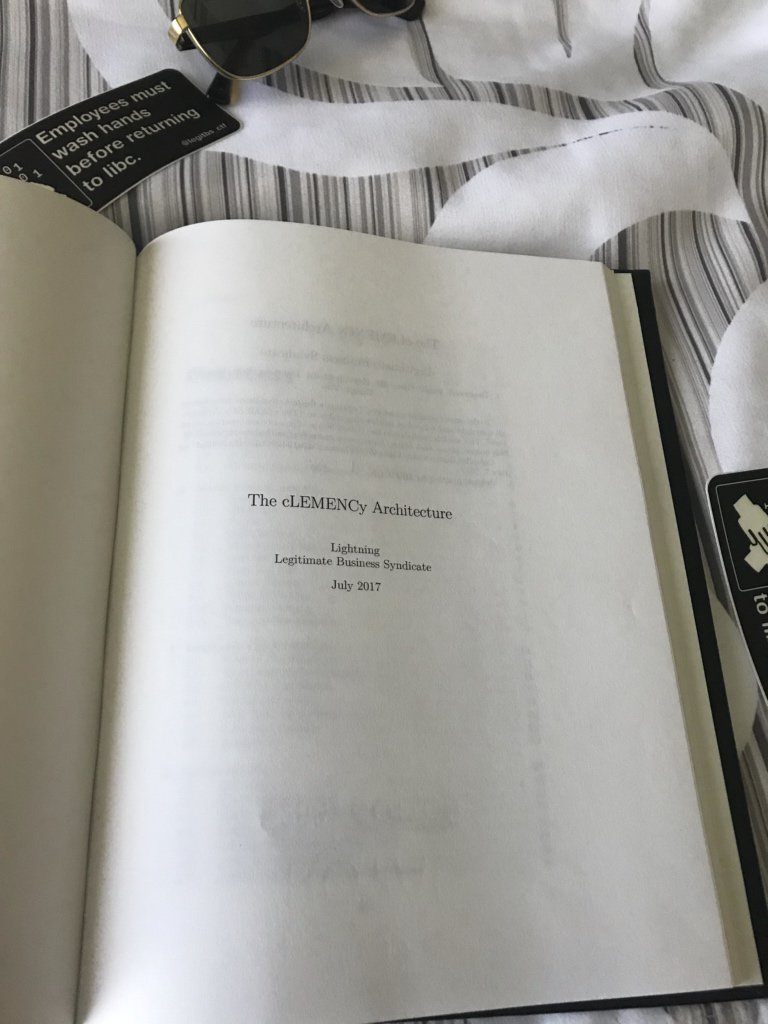
\includegraphics[height=6cm]{manual.jpg}
  \end{center}
\end{frame}

\begin{frame}[fragile]
  \frametitle{clemency-emu}
  \scriptsize
  \begin{Verbatim}[commandchars=\\\{\}]
\textcolor{magenta}{% cLEMENCy/cLEMENCy-emu/clemency-emu-debug -d 0 hello.bin}
\textcolor{blue}{> t}  # step
R00: 0000000    R01: 0000019    R02: 0000002    R03: 0000007
R04: 0000000    R05: 0000000    R06: 0000000    R07: 0000000
R08: 0000000    R09: 0000000    R10: 0000000    R11: 0000000
R12: 0000000    R13: 0000000    R14: 0000000    R15: 0000000
R16: 0000000    R17: 0000000    R18: 0000000    R19: 0000000
R20: 0000000    R21: 0000000    R22: 0000000    R23: 0000000
R24: 0000000    R25: 0000000    R26: 0000000    R27: 0000000
R28: 0000000     ST: 0000000     RA: 0000000     PC: 0000006
 FL: 0000000

0000006:                         5200780         smp    R00, R01, E
\textcolor{blue}{> db 2 3}  # hexdump
0000002: 040 001 000
\textcolor{blue}{> u 0 2}  # disassemble
0000000:                         2b0402000002b8  ldt    R01, [R00 + 0x57, 3]
0000006:                         5200780         smp    R00, R01, E
  \end{Verbatim}
\end{frame}

\begin{frame}{Instructions}
  \begin{itemize}
  \item 2,3,4,6 nytes
  \item \texttt{AD r0, r1, r2  \# ADd}
  \item \texttt{ADCI r0, r1, -4  \# ADd Immediate with Carry}
  \item \alert{M}-suffixed instructions: \alert{adjacent registers} as a pair
  \item \texttt{DVS\alert{M} r3, r27, r31  \# r3:r4 = (r27<<27 | r28) / (r31<<27 | r0)}
  \item \texttt{LD[S\alert{WT}]  \# LoaD 1/2/3 nytes, middle-endian}
  \item \texttt{ST[S\alert{WT}]  \# STore 1/2/3 nytes, middle-endian}
  \end{itemize}
\end{frame}

\begin{frame}{Middle-endian}
  \alert{W}ord of 2 nytes: \mintinline{c}{a[1] << 9 | a[0]}

  \begin{center}
    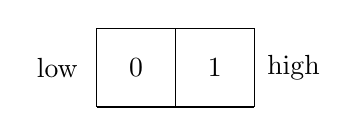
\begin{tikzpicture}
      \draw (0, 0) grid (2, 1);
      \node at (-0.5, 0.5) {low};
      \node at (0.5, 0.5) {0};
      \node at (1.5, 0.5) {1};
      \node at (2.5, 0.5) {high};
    \end{tikzpicture}
  \end{center}

  \alert{T}ri-word of 3 nytes: \mintinline{c}{a[1] << 27 | a[2] << 18 | a[0]}

  \begin{center}
    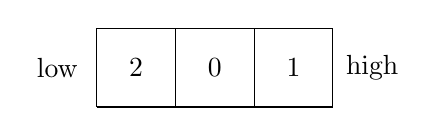
\begin{tikzpicture}
      \draw (0, 0) grid (3, 1);
      \node at (-0.5, 0.5) {low};
      \node at (0.5, 0.5) {2};
      \node at (1.5, 0.5) {0};
      \node at (2.5, 0.5) {1};
      \node at (3.5, 0.5) {high};
    \end{tikzpicture}
  \end{center}
\end{frame}

\begin{frame}{Instruction decoding}
  \footnotesize
  \begin{center}
    Instructions consist of 3-nyte groups, with permutation in each group \\
    Opcode in high bits
  \end{center}

  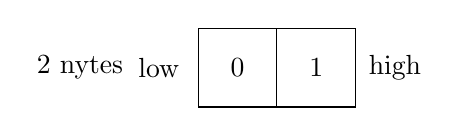
\begin{tikzpicture}
    \begin{scope}
      \draw (0, 0) grid (2, 1);
      \node at (-1.5, 0.5) {2 nytes};
      \node at (-0.5, 0.5) {low};
      \node at (0.5, 0.5) {0};
      \node at (1.5, 0.5) {1};
      \node at (2.5, 0.5) {high};
    \end{scope}
  \end{tikzpicture}

  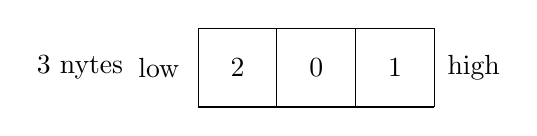
\begin{tikzpicture}
    \begin{scope}
      \draw (0, 0) grid (3, 1);
      \node at (-1.5, 0.5) {3 nytes};
      \node at (-0.5, 0.5) {low};
      \node at (0.5, 0.5) {2};
      \node at (1.5, 0.5) {0};
      \node at (2.5, 0.5) {1};
      \node at (3.5, 0.5) {high};
    \end{scope}
  \end{tikzpicture}

  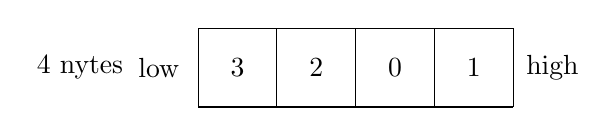
\begin{tikzpicture}
    \begin{scope}
      \draw (0, 0) grid (4, 1);
      \node at (-1.5, 0.5) {4 nytes};
      \node at (-0.5, 0.5) {low};
      \node at (0.5, 0.5) {3};
      \node at (1.5, 0.5) {2};
      \node at (2.5, 0.5) {0};
      \node at (3.5, 0.5) {1};
      \node at (4.5, 0.5) {high};
    \end{scope}
  \end{tikzpicture}

  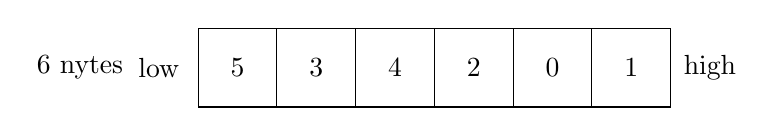
\begin{tikzpicture}
    \begin{scope}
      \draw (0, 0) grid (6, 1);
      \node at (-1.5, 0.5) {6 nytes};
      \node at (-0.5, 0.5) {low};
      \node at (0.5, 0.5) {5};
      \node at (1.5, 0.5) {3};
      \node at (2.5, 0.5) {4};
      \node at (3.5, 0.5) {2};
      \node at (4.5, 0.5) {0};
      \node at (5.5, 0.5) {1};
      \node at (6.5, 0.5) {high};
    \end{scope}
  \end{tikzpicture}
\end{frame}

\begin{frame}[fragile]
  \frametitle{Memory mappings}
  \footnotesize
  \begin{verbatim}
[0000000,4000000) Main Program Memory
[4000000,400001e) Clock IO
[4010000,4011000) Flag IO   # Capture the Flag!
[5000000,5002000) Data Received
[5002000,5002003) Data Received Size
[5010000,5012000) Data Sent
[5012000,5012003) Data Sent Size
[5100000,5104000) NFO file
[7ffff00,7ffff1c) Interrupt Pointers
[7ffff80,8000000) Processor Identification and Features
  \end{verbatim}
  \begin{center}
    \Large left-closed right-open intervals are convenient
  \end{center}
\end{frame}

\begin{frame}{radare2 plugins}
  \begin{itemize}
    \item \url{https://github.com/MaskRay/r2cLEMENCy}
    \item \texttt{io\_9bit.so}: IO
    \item \texttt{core\_clcy.so}: custom commands
    \item \texttt{bin\_clcy.so}: loader
    \item \texttt{asm\_clcy.so}: (dis)assembler
    \item \texttt{anal\_clcy.so}: instruction semantics and emulation
    \item \texttt{parse\_clcy.so}: C-like pseudo disassembler and \texttt{asm.varsub}
    \item More plugin types in \texttt{core/libs.c:r\_core\_loadlibs\_init}
    \item language, filesystem, debugger, debugger breakpoint, egg
  \end{itemize}
\end{frame}

\begin{frame}{1 nyte = 9 bits}
  \begin{center}
    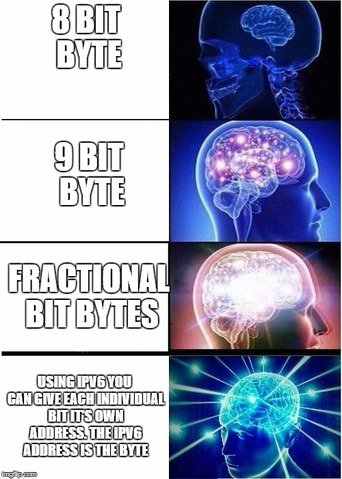
\includegraphics[height=6cm]{9-bit.jpg}
  \end{center}
  \begin{center}
    \Large Expand 1 nyte to 16-bit unsigned short
  \end{center}
\end{frame}

\begin{frame}[fragile]
  \frametitle{r\_io\_plugin\_clcy}
  \scriptsize
  \begin{minted}{c}
RIOPlugin r_io_plugin_clcy = {
  .name = "clcy",
  .desc = "cLEMENCy io",
  .license = "LGPL3",
  .check = _check,
  .close = _close,
  .extend = _extend,
  .lseek = _lseek,
  .open = _open,
  .read = _read,
  .write = _write,
};
  \end{minted}
\end{frame}

\begin{frame}{io\_clcy}
  \begin{itemize}
  \item \texttt{.open}: file $\rightarrow$ 9-bit units $\rightarrow$ 16-bit units (2 bytes)
  \item \mintinline{c}{len = len_bytes*8/9; buf = malloc(len*2);}
  \item One \alert{address unit} has 2 bytes \mintinline{c}{io->addrbytes = 2; // RIO::addrbytes}
  \item \texttt{len} argument in \texttt{read/write} still refers to bytes, not 16-bit
  \item Make sure buffers used by read()/write() are aware of \mintinline{c}{RIO::addrbytes}
  \item \texttt{.close}: 16-bit $\rightarrow$ 9-bit $\rightarrow$ file
  \end{itemize}
\end{frame}

\begin{frame}[fragile]
  \frametitle{RIO::addrbytes}
  \scriptsize
  \begin{minted}{c}
// A buffer of length RCore::blocksize (default: 256) contains
// blocksize/addrbytes (256/2=128) address units

// Before (every address unit is 1 byte):
while (idx < len) {
  r_anal_op (anal, &op, addr + idx, buf + idx,
      len - idx);

// After (buf access is aware of RIO::addrbytes):
while (addrbytes * idx < len) {
  r_anal_op (anal, &op, addr + idx, buf + addrbytes * idx,
      len - addrbytes * idx);
  \end{minted}
\end{frame}

\begin{frame}{Call path of a user command}
  \begin{itemize}
  \item \mintinline{c}{r_core_prompt_exec}
  \item \mintinline{c}{r_core_cmd}
  \item \mintinline{c}{r_core_subst}(\texttt{;},repeat,comment)
  \item \mintinline{c}{r_core_subst_i}
  \item \mintinline{c}{r_core_subst_i}(\texttt{@},backquotes,double quotes,grep,pipe,redirection)
  \item \mintinline{c}{r_cmd_call}
  \item \mintinline{c}{RCorePlugin::call} / builtin commands (\mintinline{c}{RCore.cmds.cmd['p']})
  \end{itemize}
\end{frame}

\begin{frame}[fragile]
  \frametitle{r\_core\_plugin\_clcy}
  \scriptsize
  \begin{minted}{c}
RCorePlugin r_core_plugin_clcy = {
  .name = "clcy",
  .desc = "cLEMENCy core",
  .license = "LGPL3",
  .call = r_cmd_clcy,
};

static int r_cmd_clcy(struct r_core_t *core, const char *input) {
  if (input[0] == '_') {
    ...
    case 'x': hexdump_9byte (core, input, l); break; // "_px"
    case 'w': hexdump_18word (core, input, l); break; // "_pw"
    case 't': hexdump_27tri (core, input, l); break; // "_pt"
    ...
    return true;
  }
  return false;
}
  \end{minted}
\end{frame}

\begin{frame}{bin\_clcy}
  \begin{itemize}
  \item Create sections according to cLEMENCy memory mappings
  \item \mintinline{c}{.add=true, .name="Main", .paddr=0, .size=sz,}
  \item \mintinline{c}{.vsize=0x4000000, .srwx=R_IO_READ|R_IO_EXEC}
  \item Simple IO Layer creates two \mintinline{c}{RIOMap}
  \item file map $[0, size)$ + null map $[size, vsize)$
  \end{itemize}
\end{frame}

\begin{frame}[fragile]
  \frametitle{om}
  \scriptsize
  \begin{verbatim}
[Main_Program_Memory:0x00000000]> om
10 fd: 3 +0x00000000 0x00000000 - 0x00006b67 -r-x fmap.Main_Program_Memory
 9 fd: 12 +0x00000000 0x00006b68 - 0x03ffffff -r-x mmap.Main_Program_Memory
 8 fd: 11 +0x00000000 0x00000000 - 0x0000001d -rw- mmap.Clock_IO
 7 fd: 10 +0x00000000 0x04010000 - 0x04010fff -r-- mmap.Flag_IO
 6 fd: 9 +0x00000000 0x05000000 - 0x05001fff -rw- mmap.Data_Received
 5 fd: 8 +0x00000000 0x05002000 - 0x05002001 -rw- mmap.Data_Received_Size
 4 fd: 7 +0x00000000 0x05010000 - 0x05011fff -rw- mmap.Data_Sent
 3 fd: 6 +0x00000000 0x05012000 - 0x05012001 -rw- mmap.Data_Sent_Size
#2 fd: 5 +0x00000000 0x05100000 - 0x05103fff -r-x mmap.NFO
 1 fd: 4 +0x00000000 0x07ffff00 - 0x07ffff1b -rw- mmap.Interrupt_Pointers
  \end{verbatim}
  \begin{center}
    Main Program Memory has both file map (\texttt{fmap.}) and null map (\texttt{mmap.})
  \end{center}
\end{frame}

\begin{frame}[fragile]
  \frametitle{r\_bin\_plugin\_clcy}
  \scriptsize
  \begin{minted}{c}
RBinPlugin r_bin_plugin_clcy = {
  .name = "clcy",
  .desc = "cLEMENCy bin plugin",
  .license = "LGPL3",
  .baddr = _baddr,
  .check_bytes = _check_bytes,
  .create = _create,
  .destroy = _destroy,
  .info = _info,
  .load = _load,
  .minstrlen = 0,
  .patch_relocs = _patch_relocs,
  .sections = _sections,
};
  \end{minted}
\end{frame}

\begin{frame}{bin\_clcy}
  \begin{itemize}[<+->]
  \item How to initialize NFO?
  \item \texttt{.patch\_relocs}
  \item Patch relocations in ELF/bFLT/CGC (Cyber Grand Challenge), especially
    useful for \texttt{ET\_REL}
  \item Abuse it: create and initialize a \texttt{malloc://} map
  \end{itemize}
\end{frame}

\begin{frame}[fragile]
  \frametitle{bin\_clcy \_patch\_relocs}
  \scriptsize
  \begin{minted}{c}
static RList *_patch_relocs(RBin *b) {
  ...
  RIOSection sec = {.name = "NFO", .size = n_buf * 2, .vsize = 0x4000,
    .flags = R_IO_READ | R_IO_EXEC};
  (void)r_io_create_mem_map (b->iob.io, &sec, NFO_VADDR, false);
  (void)r_io_write_at (b->iob.io, NFO_VADDR, (const ut8 *)buf, len * 2);
  ...
}
  \end{minted}
\end{frame}

\begin{frame}{asm\_clcy}
  \begin{itemize}
    \item IDA Pro processor in the game, \texttt{processor\_t.\{ana,out\}}
    \item disassembler
    \item assembler
    \item \url{https://github.com/pwning/defcon25-public} by Plaid Parliament of Pwning
    \item X macros
  \end{itemize}
\end{frame}

\begin{frame}[fragile]
  \frametitle{r\_asm\_plugin\_clcy}
  \scriptsize
  \begin{minted}{c}
static RAsmPlugin r_asm_plugin_clcy  = {
  .name = "clcy",
  .desc = "cLEMENCy asm",
  .arch = "clcy",
  .license = "LGPL3",
  .bits = 64, // in accordance with r_anal_plugin_clcy
  .disassemble = _disassemble,
  .assemble = _assemble,
};
  \end{minted}
\end{frame}

\begin{frame}[fragile]
  \frametitle{asm\_clcy struct inst\_t}
  \scriptsize
  \begin{minted}{c}
typedef struct {
  ut64 code, opcode;
  int id, size;
  ut32 pc, funct;
  st32 imm;
  ut16 cc, reg_count;
  ut8 adj_rb, arith_signed, is_imm, mem_flags, rA, rB, rC, rw, uf;
} inst_t;
  \end{minted}
\end{frame}

\begin{frame}[fragile]
  \frametitle{asm\_clcy disassembler}
  \scriptsize
  \begin{minted}{c}
// Group instructions by forms
do {
  FORMAT( R )  // assume this is an R-form instruction
  // If funct == 0b0000000 && arith_signed == 0 && is_imm == 0
  // This is ad --> break
  INS_3( ad, 0b0000000, funct, 0, arith_signed, 0, is_imm, 0 )
  // Try adc
  INS_3( adc, 0b0100000, funct, 0, arith_signed, 0, is_imm, 0 )
  // Try others
  ...
  FORMAT( R_IMM )  // assume this is an R_IMM-form instruction
  INS_2( adci, 0b0100000, arith_signed, 0, is_imm, 1 )
  ...
} while (0);

#define FORMAT(fmt) ok = decode_##fmt ...
#define INS_1(x,opc,f1,v1) if (inst.opcode==opc && inst.f1==v1) ...
#define INS_2(x,opc,f1,v1,f2,v2) if (inst.opcode==opc && inst.f1==v1 && \
  inst.f2==v2) ...
  \end{minted}
\end{frame}

\begin{frame}{pdf}
  \begin{center}
    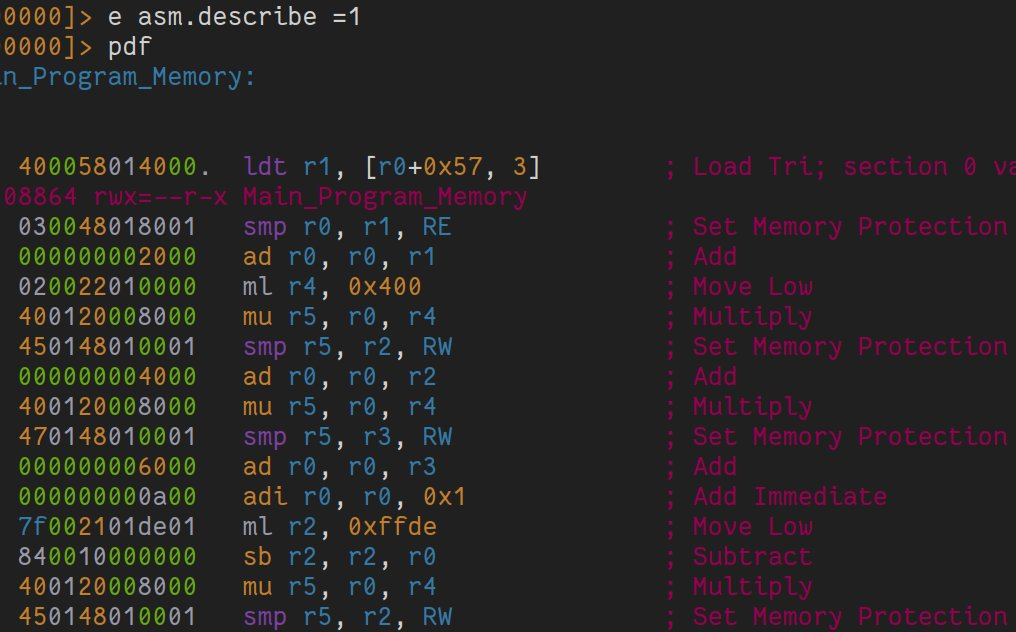
\includegraphics[height=6cm]{pdf.jpg}
  \end{center}
  \begin{center}
    Descriptions: \texttt{asm/d/clcy.sdb}
  \end{center}
\end{frame}

\begin{frame}{asm\_clcy assembler}
  \begin{itemize}
  \item \texttt{"wa ldt r1, [r0+0x57, 7]; ad. r0,r1,r1"}
  \item Recursive descent parser: \texttt{parse\_\{imm,rA,rB,rC,uf,comma,space,\ldots\}}
  \item Reuse X macros in disassembler
  \end{itemize}

  \begin{center}
    Suggest using a recursive descent parser in command parsing
  \end{center}
\end{frame}

\begin{frame}[fragile]
  \frametitle{asm\_clcy assemble\_BIN\_R\_IMM}
  \scriptsize
  \begin{minted}{c}
#define FIELD(name, offset, count) | ((ut64)inst->name << \
  bit_size-count-offset)
#define FORM_BIN_R_IMM \
  FIELD(opcode, 0, 8) \
  FIELD(rA, 8, 5) \
  FIELD(imm, 13, 14)

static int assemble_BIN_R_IMM(inst_t *inst, const char **src) {
  int bit_size = 27;
  if (parse_space (inst, src)) return 1; // parse error
  if (parse_rA (inst, src)) return 1;
  if (parse_comma (inst, src)) return -1;
  if (parse_imm_st (inst, src, 14)) return 2;
  inst->imm &= (1 << 14) - 1;
  if (parse_end (src)) return 2;
  inst->size = 3; // 3 nytes
  inst->code = 0 FORM_BIN_R_IMM; // assemble all components
  return 0;
}
  \end{minted}
\end{frame}

\begin{frame}{wa}
  \begin{center}
    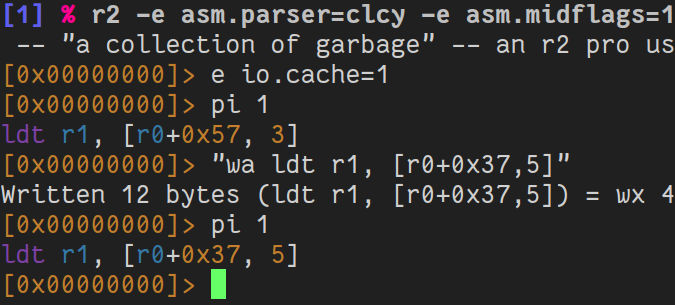
\includegraphics[width=\linewidth]{wa.jpg}
  \end{center}
\end{frame}

\begin{frame}{anal\_clcy}
  \begin{itemize}
  \item IDA Pro processor in the game, \texttt{processor\_t.emu}
  \item Differentiate \texttt{JMP/CALL/MOV/PUSH/RET/SWI/\ldots}, whether \texttt{COND,IND,MEM,REG,\ldots} are used
  \item \texttt{R\_ANAL\_OP\_TYPE\_\{JMP,COND,RCALL,RJMP,CRET,\ldots\}}
  \item \texttt{include/r\_anal.h anal/p/anal\_gb.c}
  \item Stack pointer delta (arguments, local variables), \texttt{add\_stkpnt}
  \item ESIL translator
  \end{itemize}
\end{frame}

\begin{frame}{ESIL}
  \begin{itemize}
  \item {\color{red}E}valuable {\color{red}S}trings {\color{red}I}ntermedate {\color{red}L}anguage
  \item \texttt{anal/esil.c}
  \item Stack-oriented, Forth, DWARF expressions
  \item \texttt{mh r0, 0xffdf: 0x3ff,r0,\&,10,65503,<<,|,r0,=}
  \item Decent support for 32/64 bits, needing work for 8/16 bits
  \item What if 27-bit/54-bit (register pair) + middle-endian?
  \end{itemize}
\end{frame}

\begin{frame}{anal\_clcy ESIL}
  \begin{itemize}
  \item Just set \texttt{RAnal::bits} to 64 and define custom commands (\texttt{r\_anal\_esil\_set\_op})
  \item \texttt{binop}: another argument for variants (carry/multi reg/imm/signedness/update
    flags) + instruction family (add/sub/\ldots)
  \item \texttt{addcm. r3,r2,r0} : \mintinline{c}{"r0,r2,r3,'.cm+,binop"}
  \item \alert{\texttt{'.cm+}}
  \item \texttt{'} no special, arbitrary character borrowed from Lisp
  \item \texttt{.} update flags
  \item \texttt{c} with carry
  \item \texttt{+} add
  \end{itemize}
\end{frame}

\begin{frame}[fragile]
  \frametitle{clcy\_custom\_binop}
  \scriptsize
  \begin{minted}{c}
r_anal_esil_set_op (esil, "binop", clcy_custom_binop);

static int clcy_custom_binop(RAnalEsil *esil) {
  bool carry = false, uf = false, mf;
  char *op = r_anal_esil_pop (esil), *op1 = op + 1,
    *rA = r_anal_esil_pop (esil), *rB = r_anal_esil_pop (esil),
    *rC = r_anal_esil_pop (esil);
  ...
  if (*op1 == '.') uf = true, op1++; // .: update flags
  if (*op1 == 'c') carry = true, op1++; // c: carry
  if (*op1 == 'm') ... // m: multi reg
  switch (*op1) {
  case '+': a = b + c; if (carry && read_fl (esil) & 2) a++; ...
  case '-': ...
  }
  if (uf) { /* update Carry/Overflow/Sign/Zero flags */ }
  ...
}
  \end{minted}
\end{frame}

\begin{frame}{Local variables/arguments detection}
  \begin{itemize}
    \item Analysis engine detects with patterns like \texttt{0x..,st,+}
    \item We have custom \texttt{load/store} commands to emulate
      \texttt{LD[STW], ST[STW]}
    \item No-op \mintinline{c}{0x34,st,+,POP} to appease analysis engine
  \end{itemize}
\end{frame}

\begin{frame}[fragile]
  \frametitle{RAnalPlugin}
  \scriptsize
  \begin{minted}{c}
static RAnalPlugin r_anal_plugin_clcy = {
  .name = "clcy",
  .desc = "cLEMENCy analysis",
  .license = "LGPL3",
  .arch = "clcy",
  .bits = 64, // we use 64-bit integers in esil to emulate 27-bit and 54-bit
  .esil_init = esil_clcy_init,
  .esil_fini = esil_clcy_fini,
  .esil_intr = esil_clcy_intr,
  .esil = true,
  .op = &clcy_op,
  .set_reg_profile = set_reg_profile,
};
  \end{minted}
\end{frame}

\begin{frame}{VV}
  \begin{center}
    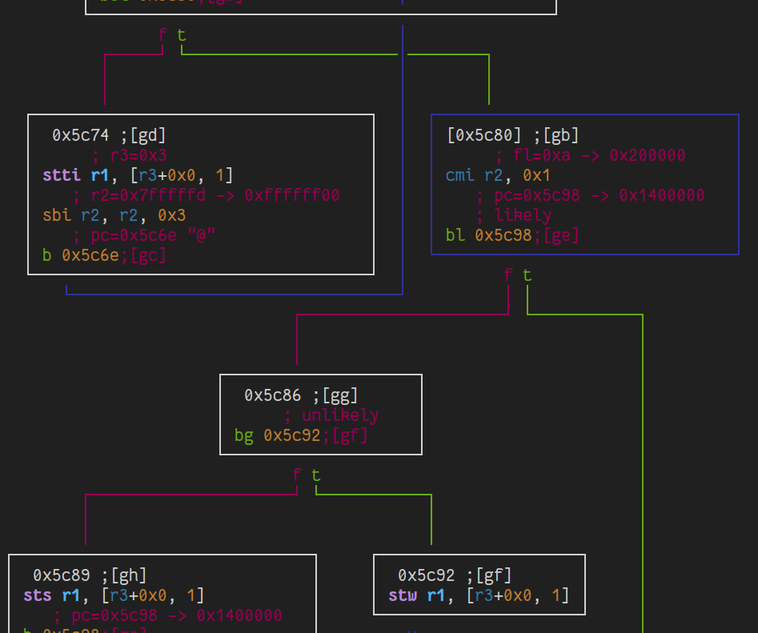
\includegraphics[height=7cm]{graph.png}
  \end{center}
\end{frame}

\begin{frame}{parse\_clcy}
  \begin{itemize}
  \item Bad name \url{https://github.com/radare/radare2/issues/4317}
  \item How to substitue variables for BP/SP offsets: \texttt{asm.varsub}
  \item How to generate C-like pseudo disassembly: \texttt{pdc}
  \end{itemize}
\end{frame}

\begin{frame}[fragile]
  \frametitle{r\_parse\_plugin\_clcy}
  \scriptsize
  \begin{minted}{c}
static int _parse(RParse *p, const char *src, char *dst);
static bool _varsub(RParse *p, RAnalFunction *f, ut64 addr,
  int oplen, char *src, char *dst, int len);

RParsePlugin r_parse_plugin_clcy = {
  .name = "clcy",
  .desc = "cLEMENCy",
  .parse = _parse,
  .varsub = _varsub,
};
  \end{minted}
\end{frame}

\begin{frame}[fragile]
  \frametitle{parse\_clcy \_parse}
  \scriptsize
  \begin{minted}{c}
static int _parse(RParse *p, const char *src, char *dst) {
  RCore *core = p->user;
  RAsmOp op;
  int len;
  // `assemble` could be saved if we had access to metadata of previous
  // call to `assemble`
  if ((len = assemble (core->assembler->pc, &op, src)) > 0 &&
      disassemble (core->assembler->pc, &op, op.buf, len, true) > 0) {
    strcpy (dst, op.buf_asm);
  } else {
    strcpy (dst, src);
  }
  return true;
}
  \end{minted}
\end{frame}

\begin{frame}{pdc}
  \begin{center}
    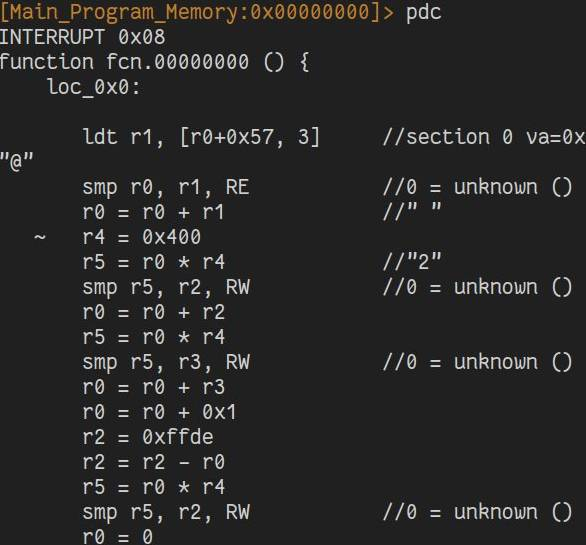
\includegraphics[height=7cm]{pdc.jpg}
  \end{center}
\end{frame}

\begin{frame}[fragile]
  \frametitle{parse\_clcy \_varsub}
  \scriptsize
  \begin{minted}{c}
static bool _varsub(RParse *p, RAnalFunction *f, ut64 addr, int oplen,
    char *src, char *dst, int len) {
  ...
  // Stack register variable st+%#x
  r_list_foreach (bpargs, iter, var) {
    if (var->delta >= 0) {
      sub = r_str_newf ("[st+%#x", var->delta);
    } else {
      sub = r_str_newf ("[st-%#x", -var->delta);
    }
    // replace sub with var->name
  ...
}
  \end{minted}
\end{frame}

\begin{frame}{asm.varsub}
  \begin{center}
    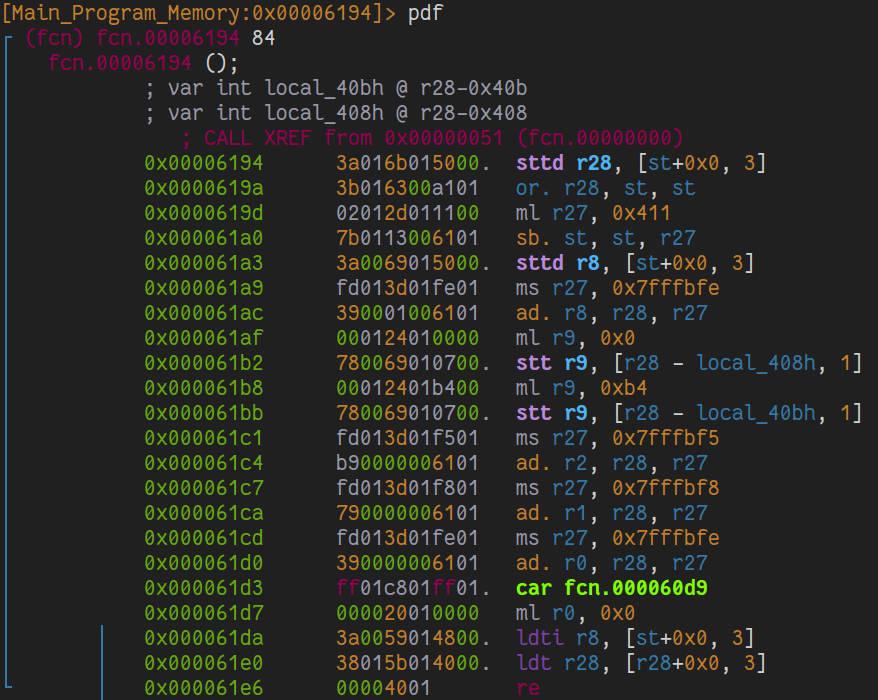
\includegraphics[height=6cm]{varsub.jpg}
  \end{center}
  \begin{center}
    \large See \texttt{local\_*} variables. 0 offset is not handled currently
  \end{center}
\end{frame}

\begin{frame}{debug\_clcy}
  \begin{center}
    \Large Left as exercise.
  \end{center}
\end{frame}

\begin{frame}
  \begin{center}
    \Large \url{https://github.com/MaskRay/r2cLEMENCy}
  \end{center}
  \begin{center}
    \Large Questions?
  \end{center}
\end{frame}

\end{document}
